\documentclass[fleqn,10pt,serif,xcolor=svgnames,xcolor=table,aspectratio=169,handout]{beamer}
% \includeonlyframes{current}
%========================================
% Packages
%========================================

\usepackage[palatino]{../../99-auxiliary-files/00-mypackBeamer}
\usepackage{../../99-auxiliary-files/00-mycommands}
\usepackage{../../99-auxiliary-files/00-myenvironments-beamer}

\usepackage{tikz-qtree}
\usepackage{array}
\usepackage[absolute,overlay]{textpos}
\usepackage{ulem}

%========================================
% More Layout (Beamer Special)
%========================================

\DefineNamedColor{named}{mycol}{cmyk}{0.6,0.6,0,0}
% \DefineNamedColor{named}{mygray}{cmyk}{0.05,0.05,0.05,0.05}
% \DefineNamedColor{named}{mygraylight}{cmyk}{0.017,0.017,0.017,0.017}

\definecolor{signal1}{rgb}{0.69, 0.25, 0.21}
\definecolor{signal2}{rgb}{1.0, 0.66, 0.07}
\definecolor{signal3}{rgb}{0.39, 0.58, 0.93}
\definecolor{signal4}{rgb}{0.0, 0.4, 0.0}
\definecolor{firebrick}{rgb}{0.7, 0.13, 0.13}
\definecolor{themecolor}{rgb}{0.3, 0.36, 0.33} % feldgrau
\definecolor{darkgray}{rgb}{0.66, 0.66, 0.66}

% \usetheme[height=7mm]{Rochester}
%\usetheme{Warsaw}


\usecolortheme{dove}

% \useoutertheme[compress,subsection=false]{miniframes}

\usecolortheme[named=themecolor]{structure}

\setbeamercolor{title}{fg=themecolor}

% \setbeamercolor{lower separation line head}{bg=white}

%\setbeamercolor{structure}{fg=Brown}
%\setbeamercolor{normal text}{fg=Brown}
%\setbeamercolor{section in head/foot}{bg=gray!40}
%%\setbeamercolor{lower separation line head}{bg=black!40}
%\setbeamercolor*{frametitle}{fg=Black,bg=gray!40}
%\setbeamercolor*{block body}{fg=Brown,bg=gray!00}
%\setbeamercolor*{block title}{fg=Black,bg=gray!40}


% Switch of shadows of boxes
\setbeamertemplate{blocks}[default]

% Frame numbers in footer
\setbeamertemplate{footline}[frame number]

% See-through preview for uncovered
% \setbeamercovered{transparent}

% Switch off navigation panel at bottom right
\beamertemplatenavigationsymbolsempty

% Change Style for itemize markers
% Options are ball, circle, rectangle and default (=triangle)
\setbeamertemplate{items}[circle]



\setcounter{tocdepth}{1}

% Use bullets in enumerates and TOC
\setbeamertemplate{enumerate item}[circle]

% Set color for enumerate/TOC bullets to white
\setbeamercolor*{item projected}{fg=themecolor,bg=gray!00}

\setbeamercolor*{author}{fg=gray!80}

\setbeamerfont*{block title}{size=\normalsize}
\setbeamerfont*{title}{size=\huge}
\setbeamerfont*{subtitle}{size=\large}

% \newcommand{\mygray}[1]{{\color{gray}{#1}}}
% \newcommand{\mycol}[1]{{\color{mycol}{#1}}}

\newcommand{\mycomment}[1]{\hfill {\mygray{#1}}}
\newcommand{\mycom}[1]{\hfill {\mygray{[#1]}}}

\newcommand{\slideFN}[1]{%
  \begin{textblock*}{\paperwidth}(0pt,1.05\textheight)
    \hfill \footnotesize{\mygray{#1}} \hspace{.5em}
  \end{textblock*}}

\newcommand{\pictureslide}[2][current]{
\usebackgroundtemplate{\includegraphics[width=\paperwidth]{#2}}%
\begin{frame}[label=#1]

\end{frame}
}
% code below makes it possible to turn inclusion of frames
% into 'miniframes' off and on with commands:
% \miniframeson and \miniframesoff
% from: http://tex.stackexchange.com/questions/37127/how-to-remove-some-pages-from-the-navigation-bullets-in-beamer

\makeatletter
\let\beamer@writeslidentry@miniframeson=\beamer@writeslidentry
\def\beamer@writeslidentry@miniframesoff{%
  \expandafter\beamer@ifempty\expandafter{\beamer@framestartpage}{}% does not happen normally
  {%else
    % removed \addtocontents commands
    \clearpage\beamer@notesactions%
  }
}
\newcommand*{\miniframeson}{\let\beamer@writeslidentry=\beamer@writeslidentry@miniframeson}
\newcommand*{\miniframesoff}{\let\beamer@writeslidentry=\beamer@writeslidentry@miniframesoff}
\makeatother

\setbeamertemplate{bibliography item}{}


%========================================
% Commands
%========================================

\newcommand{\mycol}[1]{{\textcolor{mycol}{#1}}}
\renewcommand{\markdef}[1]{\mycol{#1}}
\newcommand{\mygray}[1]{\textcolor{gray}{#1}}
\definecolor{darkgray}{rgb}{0.66, 0.66, 0.66}

\renewcommand{\slideFN}[1]{%
  \begin{textblock*}{\paperwidth}(0pt,0.95\textheight)
    \hfill \footnotesize{\mygray{#1}} \hspace{.5em}
  \end{textblock*}}

\newcommand{\proplog}{\acro{PropLog}}
\newcommand{\predlog}{\acro{PredLog}}

\def\checkmark{\tikz\fill[scale=0.4](0,.35) -- (.25,0) -- (1,.7) -- (.25,.15) -- cycle;}

%========================================
% Document
%========================================

\title{Predicate logic}
\subtitle{Methods: Logic, Part 5}

\author{Michael Franke}
\date{}


%--------------------------------------

\begin{document}

% --- Horizontal Space Fix ----

\abovedisplayskip=3pt
\abovedisplayshortskip=3pt

\belowdisplayskip=3pt
\belowdisplayshortskip=3pt

\begin{frame}
  \maketitle
\end{frame}

\begin{frame}
  % \frametitle{From propositional to predicate logic}

  \bigskip

  \begin{minipage}{0.45\linewidth}
    \begin{center}
      \textcolor{themecolor}{\textbf{Dumbo}}
      
\includegraphics[height=2cm]{pics/dumbo-elephant.png}
    \end{center}
  \end{minipage}
  \hfill
  \begin{minipage}{0.45\linewidth}
    \begin{center}
      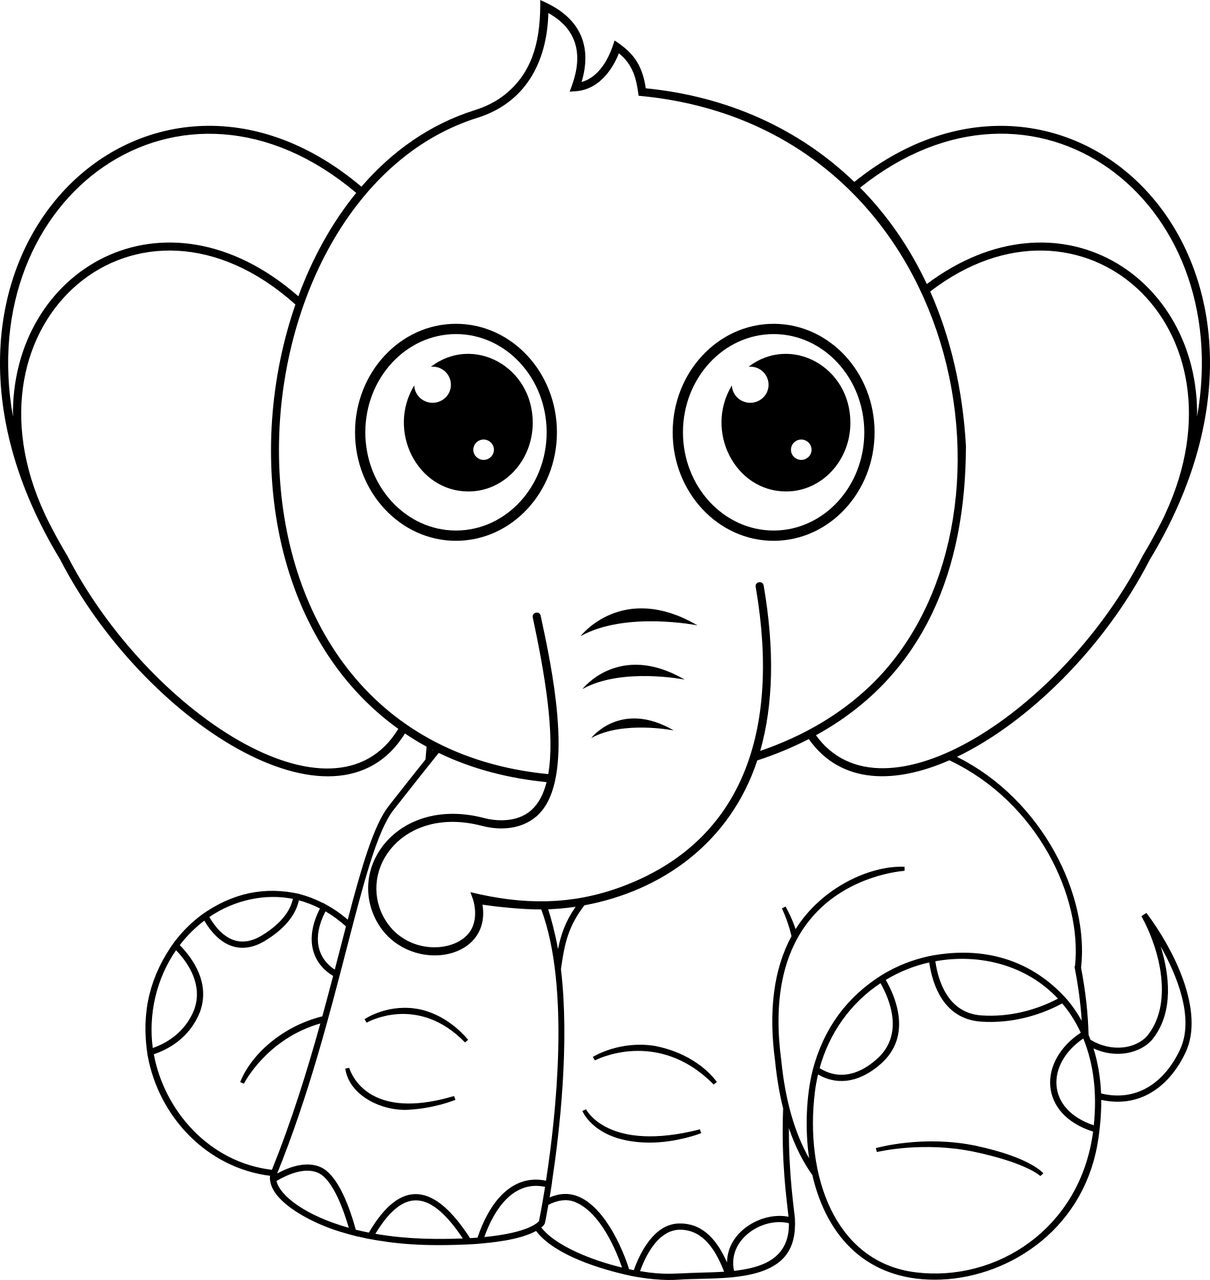
\includegraphics[height=2cm]{pics/kimbi-elephant.png}
      \textcolor{themecolor}{\textbf{Kimbi}}
    \end{center}
  \end{minipage}

  \bigskip
  \bigskip
  \pause

  \begin{center}
    \begin{tabular}[]{lcc}
      natural language
      & \proplog
      & \predlog
      \\ \midrule
      %
      \textcolor{signal1}{Dumbo} is an \textcolor{signal3}{elephant}.
      & $p$
      & $\textcolor{signal3}{E}\textcolor{signal1}{d}$
      \\
      %
      \textcolor{signal2}{Kimbi} is an \textcolor{signal3}{elephant}.
      & $r$
      & $\textcolor{signal3}{E}\textcolor{signal2}{k}$
      \\
      %
      All \textcolor{signal3}{elephants} are \textcolor{signal4}{mammals}.
      & ???
      & $\forall x \myts (\textcolor{signal3}{E}x \rightarrow \textcolor{signal4}{M}x)$
      \\
      %
      \textcolor{signal1}{Dumbo} is a \textcolor{signal4}{mammal}.
      & $q$
      & $\textcolor{signal4}{M}\textcolor{signal1}{d}$
      \\
      %
      \textcolor{signal2}{Kimbi} is a \textcolor{signal4}{mammal}.
      & $s$
      & $\textcolor{signal4}{M}\textcolor{signal2}{k}$
      \\
      %
    \end{tabular}
  \end{center}

\end{frame}

\begin{frame}
  \frametitle{Elements of the language of predicate logic}

  \begin{itemize}
    \item individual constants $a,b,c, \dots, v$
    \item predicate letters $A, B, C, D \dots$
    \item variables $w, x,y,z$
    \item parentheses ( \ \ )
    \item sentential connectives $\neg, \wedge, \vee, \rightarrow, \leftrightarrow$
    \item quantifiers $\exists, \forall$
  \end{itemize}

\end{frame}

\begin{frame}
  \frametitle{Formula of predicate logic}

  \begin{enumerate}[(i)]
    \item If $A$ is an $n$-ary predicate letter and if $t_1, \dots, t_n$ are individual constants     or variables, then $At_1 \dots t_n$ is a formula.
    \item If $\varphi$ is a formula, then so is $\neg \varphi$.
    \item If $\varphi$ and $\psi$ are formulas, so are:
    \vspace*{-0.4cm}
    \begin{multicols}{4}
      \begin{enumerate}[a.]
        \item ($\varphi \wedge \psi$)
        \item ($\varphi \vee \psi$)
        \item ($\varphi \rightarrow \psi$)
        \item ($\varphi \leftrightarrow \psi$)
      \end{enumerate}
    \end{multicols}
    \vspace*{-0.4cm}
    \item If $\varphi$ is a formula and if $x$ is a variable, then these are formulas:
    \vspace*{-0.4cm}
    \begin{multicols}{2}
      \begin{enumerate}[a.]
        \item $\forall x \myts \varphi$ \ \ \ [\textit{universal statement}]
        \item $\exists x \myts \varphi$ \ \ \ [\textit{existential statement}]
      \end{enumerate}
    \end{multicols}
    \vspace*{-0.4cm}
    \item Anything that cannot be constructed by (i)--(iv) is not a formula.
  \end{enumerate}

\end{frame}


\begin{frame}
  \frametitle{Syntactic trees}

  \begin{center}
    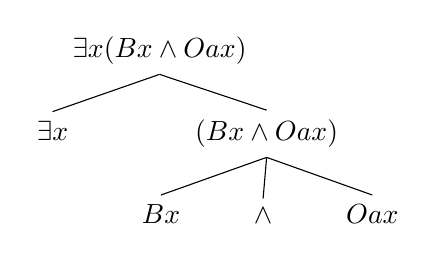
\begin{tikzpicture}[sibling distance=20pt, level distance=30pt]
      \Tree [.{$\exists x \myts (Bx \wedge Oax)$} [. $\exists x$ ] [. {$(Bx \wedge Oax)$} [. $Bx$ ] [. $\wedge$ ] [. $Oax$ ] ] ]
    \end{tikzpicture}
    \quad \quad \quad \quad \quad \quad
    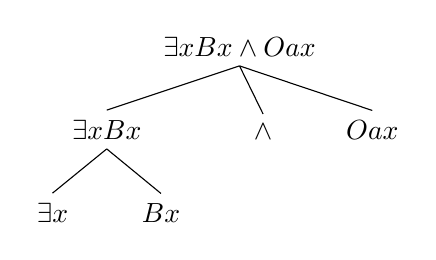
\begin{tikzpicture}[sibling distance=20pt, level distance=30pt]
      \Tree [.{$\exists x \myts Bx \wedge Oax$} [. {$\exists x \myts Bx$} [. $\exists x$ ] [. $Bx$ ] ] [. {$\wedge$} ] [. $Oax$ ] ]
    \end{tikzpicture}
  \end{center}

\end{frame}


\begin{frame}
  \frametitle{Translation}

  \begin{minipage}{0.3\linewidth}
    \textbf{Domain of quantification}
  \end{minipage}
  \hfill
  \begin{minipage}{0.65\linewidth}
      \textbf{Translation key}
\end{minipage}

\begin{minipage}{0.3\linewidth}
  \begin{itemize}
    \item[] all human beings
    \item[]
    \item[]
  \end{itemize}
  \end{minipage}
  \hfill
  \begin{minipage}{0.65\linewidth}
    \begin{multicols}{2}
    \begin{enumerate}
      \item[] $a$: Alex
      \item[] $b$: Bo
      \item[] $Fx$: $x$ is friendly
      \item[] $Lxy$: $x$ likes $y$
      \item[] $Px$: $x$ is a pilot
      \item[] $Sxy$: $x$ is a sibling of $y$
    \end{enumerate}
  \end{multicols}
\end{minipage}

\bigskip
\bigskip

\textbf{Examples}
  \begin{align*}
    & \text{Alex is a pilot.}
    && Pa
    \\
    & \text{Bo is an friendly pilot.}
    && Fb \wedge Pb
    \\
    & \text{No pilot is friendly.}
    && \forall x \myts (Px \rightarrow \neg Fx)
    \\
    & \text{Nobody likes pilots.}
    && \neg \exists x \myts \exists y \myts (Py \wedge Lxy)
    \\
    & \text{Bo has a friendly sibling.}
    && \exists x \myts (Sx \wedge Sbx)
    \\
    & \text{Every pilot has a friendly sibling.}
    && \forall x \myts (Px \rightarrow (\exists y \myts (Fy \wedge Sxy)))
  \end{align*}
\end{frame}

\end{document}
